\section{Introduction --- What Are We Building?}

Imagine you want to build a device that can represent \emph{any} mapping from two binary inputs to a binary output. You could hard-wire a specific logic gate, but then you'd have to rebuild the circuit every time you wanted a different function. What if, instead, you could build a single circuit and simply \emph{adjust some knobs} to change what it computes?

This is exactly what a \textbf{neural network} does. A neural network is a system of adjustable \emph{weights}, \emph{summers}, and \emph{cutoffs} that can be ``trained'' to represent any function. In this lab you will build one entirely from analog op-amp circuits.

\subsection*{The 2-2-1 Network}

Our network has the following structure:

\begin{center}
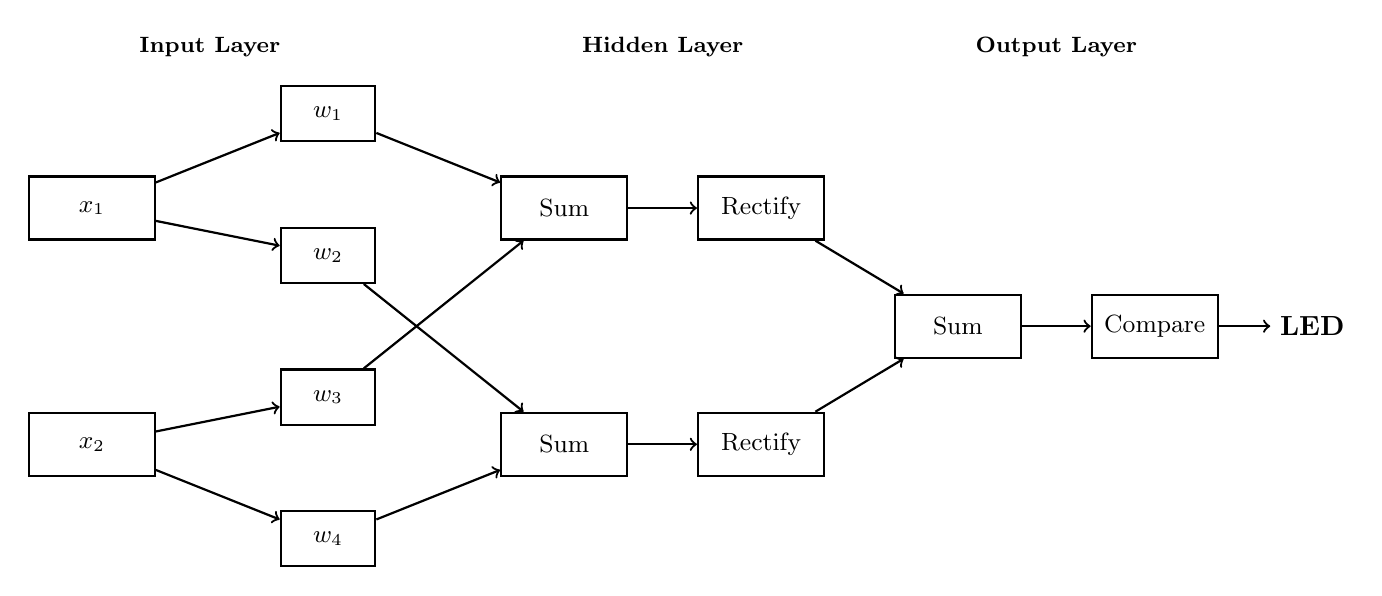
\begin{tikzpicture}[
    block/.style={draw, thick, minimum width=1.6cm, minimum height=0.8cm, align=center, font=\small},
    smallblock/.style={draw, thick, minimum width=1.2cm, minimum height=0.7cm, align=center, font=\small},
    arr/.style={->, thick},
]
% --- Column 1: Inputs ---
\node[block] (x1) at (0, 1.5) {$x_1$};
\node[block] (x2) at (0, -1.5) {$x_2$};

% --- Column 2: Weight Pots (4 boxes) ---
\node[smallblock] (w1) at (3, 2.7) {$w_1$};
\node[smallblock] (w2) at (3, 0.9) {$w_2$};
\node[smallblock] (w3) at (3, -0.9) {$w_3$};
\node[smallblock] (w4) at (3, -2.7) {$w_4$};

% --- Column 3: Summers ---
\node[block] (sum1) at (6, 1.5) {Sum};
\node[block] (sum2) at (6, -1.5) {Sum};

% --- Column 4: Rectifiers ---
\node[block] (act1) at (8.5, 1.5) {Rectify};
\node[block] (act2) at (8.5, -1.5) {Rectify};

% --- Column 5: Output Summer ---
\node[block] (sumout) at (11, 0) {Sum};

% --- Column 6: Comparator ---
\node[block] (comp) at (13.5, 0) {Compare};

% --- Column 7: LED ---
\node (led) at (15.5, 0) {\textbf{LED}};

% === Arrows: Inputs to Weight Pots (diagonal) ===
\draw[arr] (x1) -- (w1);
\draw[arr] (x1) -- (w2);
\draw[arr] (x2) -- (w3);
\draw[arr] (x2) -- (w4);

% === Arrows: Weight Pots to Summers (diagonal, crossing) ===
\draw[arr] (w1) -- (sum1);
\draw[arr] (w3) -- (sum1);
\draw[arr] (w2) -- (sum2);
\draw[arr] (w4) -- (sum2);

% === Arrows: Summers to Rectifiers (straight) ===
\draw[arr] (sum1) -- (act1);
\draw[arr] (sum2) -- (act2);

% === Arrows: Rectifiers to Output Summer (diagonal) ===
\draw[arr] (act1) -- (sumout);
\draw[arr] (act2) -- (sumout);

% === Arrows: Output Summer to Comparator to LED (straight) ===
\draw[arr] (sumout) -- (comp);
\draw[arr] (comp) -- (led);

% === Layer Labels ===
\node[font=\footnotesize\bfseries, above] at (1.5, 3.3) {Input Layer};
\node[font=\footnotesize\bfseries, above] at (7.25, 3.3) {Hidden Layer};
\node[font=\footnotesize\bfseries, above] at (12.25, 3.3) {Output Layer};

\end{tikzpicture}
\end{center}

Here is what each block does:

\begin{itemize}
    \itemsep2pt
    \item \textbf{Inputs} ($x_1$, $x_2$): Toggle switches selecting $+9$V (``on'') or $-9$V (``off'').
    \item \textbf{Weight Pots}: Potentiometers that scale each input by a value between $-1$ and $+1$. Turning the knob changes the weight.
    \item \textbf{Summers}: Op-amp circuits that add the weighted inputs together.
    \item \textbf{Rectifiers}: Diode circuits that pass only positive voltages and force negative ones to zero. This cutoff is what allows the network to make different ``decisions'' for different inputs --- without it, the whole network would just be one big addition, which is far too simple.
    \item \textbf{Comparator + Threshold}: Compares the output sum against an adjustable threshold voltage. If the sum exceeds the threshold, the LED turns on (output = 1). Otherwise, the LED is off (output = 0).
\end{itemize}

Over the rest of this lab, you will build each of these blocks as an analog circuit and then wire them together into a working neural network.

\subsection*{Dual Power Supply Setup}

Op-amps are \emph{active devices} that require external power. In this lab, we use a \emph{dual-sided supply}, providing $+9$\si{\volt} to $+V_{CC}$ and $-9$\si{\volt} to $-V_{CC}$. You can make this with two $9$V batteries connected in series:

\begin{figure}[h]
	\centering
	\begin{circuitikz}[scale=1,transform shape,american]
  	\draw (0,0) to[battery,*-o,v_=9V] (-4,0) node[anchor=south]{-$V_{CC}$};
  	\draw (4,0) node[anchor=south]{+$V_{CC}$} to[battery,o-,v_=9V] (0,0);
  	\draw (0,0) node[sground]{};
	\end{circuitikz}
	\caption{Making a dual-sided supply with two $9$V batteries}
	\label{fig:dual-sided-supply}
\end{figure}

\infotext{\linewidth}{Note the polarity of the battery terminals (connected positive to negative)}

Designate one half of your breadboard to use the $\pm 9$V rails. \textbf{Please remove the connections connecting all of your supply rails together on this section of the board.} The blue rails will be the reference node (ground), one of the red rails will be $+9$V, and the other red rail will be $-9$V. Figure \ref{fig:dual-supply-bb} is a breadboard diagram showing how to connect your batteries.

\begin{figure}[h]
	\centering
    \hspace{.5em}\includegraphics[width=0.9\linewidth]{dual-supply-bb_2.png}
	\caption{Making a dual-sided supply on a breadboard}
	\label{fig:dual-supply-bb}
\end{figure}

\warning{\linewidth}{Before connecting devices to the supply rails, check voltages with multimeter!}

Connect the black probe (COM) to the blue GND rail and you should measure +9V on one red rail and $-$9V on the other red rail. Make sure that you keep track of which is which. If you reverse the supply voltages going to the op amp chip, it can get very hot. \textbf{If the op-amp chip feels warm to the touch, disconnect the batteries immediately.}
